% TMLR manuscript for the SLEP P1-P4 pre-registered test.
% Requires the official TMLR style file tmlr.sty and tmlr.bst, obtainable from
%   https://github.com/JmlrOrg/tmlr-style-file
% Place tmlr.sty, tmlr.bst, fancyhdr.sty (if needed) alongside this file.
% Toggle the mode below: default = anonymous submission.
\documentclass{article}
\usepackage{tmlr}
% \usepackage[preprint]{tmlr}   % non-anonymous preprint
% \usepackage[accepted]{tmlr}   % camera-ready

\usepackage{amsmath,amssymb}
\usepackage{graphicx}
\usepackage{booktabs}
\usepackage{microtype}

\title{A Pre-registered Empirical Test of Four Predictions from the\\
       Semantic Least-Energy Principle: One Pass, Three Tests Not Constituted}

% Author block (fill for the non-anonymous version).
\author{\name Anonymous \email anon@example.com}

\def\month{09}  % submission month

\begin{document}
\maketitle

\begin{abstract}
The Semantic Least-Energy Principle (SLEP) states, in its prediction protocol,
four falsifiable claims: P1, energy decreases during learning and compresses
after fit; P2, inference trajectories concentrate on low-action paths; P3,
deliberation trajectories in low-gradient regions are near-geodesic; P4,
self-information is affine in the potential with an identifiable temperature.
We execute a pre-registered test of these four predictions on three small
systems (a $\beta$-VAE, a recurrent world model and a multi-step-decoder
variant, and a small Transformer sequence world model). Decision thresholds
are traced to calibration artifacts; the judging code is frozen before any
evaluation data is touched and time-stamped by a public repository commit; each
cell of the prediction $\times$ system grid receives a three-valued verdict
(\emph{pass} / \emph{fail} / \emph{test not constituted}). P2 passes on the
multi-step-decoder world model: across all five evaluation seeds the observed
Onsager--Machlup action lies below the lower quartile of an endpoint-matched
surrogate distribution, and the concentration is attributed to potential
structure by a potential-term ablation (paired difference positive, Wilcoxon
signed-rank $p$ between $10^{-12}$ and $7\times10^{-34}$). The apparent affine
law (P4) loses its evidential standing under a decoupling control (retraining
the decoder on occupancy-uniform data shifts the slope by $0.16$--$0.30$,
exceeding the pre-registered tolerance $0.12$), and its curvature effect size
exceeds the substantive-bending bound on every seed; the utility-plateau premise
of P1 holds on none of thirteen gated training instances, with post-peak entropy
rising rather than compressing; P3 does not run because the geodesic residual
quality check, calibrated on analytically smooth synthetic metrics, is not met
on estimated metrics. The test itself yields four instrument findings: a
mutual exclusion between training length and metric measurability, an
order-of-magnitude repair of latent-space geometry by a multi-step decoder head,
feasibility that is not a single-variable function of the condition number, and
non-portability of a residual-scale quality check between analytic and estimated
metrics.
\end{abstract}

\section{Introduction}

The parent theory \citep{slep_parent} proposes that a learning system with a
utility constraint descends a free energy on the learning time scale, and that
on the inference time scale its internal state approximately follows a Langevin
dynamics whose drift is a semantic potential gradient. Its prediction protocol
(Section~4.7 of the parent paper) compresses this claim into four separately
falsifiable predictions. This paper is a record of executing that protocol.

The operational content of the four predictions is as follows.
\begin{itemize}
\item \textbf{P1} (energy decreases during learning, compresses after fit): along
training checkpoints, the mean potential $\langle\hat V\rangle$ and the entropy
$\hat S$ keep decreasing after utility reaches a plateau---utility stops rising,
yet the internal representation keeps compressing.
\item \textbf{P2} (low-action concentration): the path action of an inference
trajectory is significantly below that of endpoint-, length-, and
speed-distribution-matched random surrogate paths, and this concentration is
attributed to the potential-gradient term---replacing the potential with a
constant should visibly degrade discrimination.
\item \textbf{P3} (near-geodesic in low-gradient regions): deliberation
trajectories in flat regions of the potential field are closer to the
same-endpoint geodesic than those in steep regions.
\item \textbf{P4} (affine law and temperature): the self-information $\hat I$ is
linear in the potential $\hat V$, $\hat I \approx a + b\,\hat V$, with the
temperature identified by $\hat T = 1/b$ and consistent under a split-half.
\end{itemize}

The methodological backbone has three commitments. First, threshold provenance:
every decision threshold comes from calibration measurements on synthetic
systems with known ground truth, and each constant in the code carries a comment
pointing to its derivation artifact. Second, decision freezing and external
time stamp: the judging code and threshold table are frozen before the
evaluation-family data is touched, time-stamped by a public Git commit hash;
during the evaluation phase the human role is reduced to running code. Third,
three-valued accounting: a cell that fails an admission gate (capability,
geometry, stationarity, geodesic uniqueness) is recorded as \emph{test not
constituted} and is kept statistically separate from \emph{fail}---a failure
outside the gate has no refuting force, and a pass outside the gate has no
supporting force.

\section{Systems and estimators}

\subsection{Test systems}

\textbf{S1}: a $\beta$-VAE \citep{higgins2017betavae,kingma2014vae} on dSprites
\citep{dsprites}, latent dimension $8$, $\beta\in\{1,4\}$. Ground-truth factors
are known; utility is a factor-probe composite (shape classification accuracy
and scale/x/y regression $R^2$, negatives clipped to zero, averaged).

\textbf{S2}: a GRU world model on a procedurally generated maze navigation
environment, hidden dimension $16$, two-channel local observation (walls and a
goal indicator), a per-channel fixed-variance Gaussian decoder. Utility is a
deterministic near-target navigation success rate (fixed task list, per-task
fixed random stream, so repeat noise is zero). The inference trajectory is the
evolution of the hidden state along real execution.

\textbf{S2P}: the multi-step-decoder variant of S2 (protocol v1.2 appendix)---the
decoder outputs the concatenation of the next four observations, everything else
unchanged. The design motivation is in the instrument findings
(Section~\ref{sec:multistep}).

\textbf{S3}: a small causal Transformer sequence world model (2 layers, width
$32$, 2 heads); data distribution and utility follow S2, the hidden state is the
last-layer residual stream, and the multi-step decoder head follows S2P. Per the
plan it is tested on P1 only.

\subsection{Estimators}

The metric $\hat g$ is the pull-back of the Gaussian-decoder Fisher information,
\begin{equation}
\hat g(z) = J(z)^{\top}\,\Sigma^{-1}\,J(z),
\end{equation}
where $z$ is the latent state (dimension $8$ or $16$), $J(z)$ is the Jacobian of
the decoder mean with respect to $z$ (observation dim $\times$ latent dim), and
$\Sigma$ is the diagonal covariance of the decoder observation noise. It measures
``how much the observation distribution changes when the latent state moves a
little in a given direction.''

The potential $\hat V(z)$ is the mean decoder negative log-likelihood over the
$k$-nearest-neighbours ($k=32$) of $z$; density is estimated by two paths (a
$k$-NN estimator \citep{kozachenko1987knn} and a self-written RealNVP
normalizing flow \citep{dinh2017realnvp}) for cross-validation, and the entropy
$\hat S$ likewise by two paths. The self-information carries a volume correction,
\begin{equation}
\hat I(z) = -\log\hat p(z) + \tfrac12\log\det\hat g(z),
\end{equation}
with $\hat p$ the latent density estimate. The correction converts a coordinate
density into a density relative to the invariant volume of the manifold; without
it, the two axes of the affine law depend on the parameterization. The path
action is the discretized Onsager--Machlup main term
\citep{onsager1953om},
\begin{equation}
\hat A_{\mathrm{OM}} = \frac{1}{4T}\sum_t
\big\| \Delta z_t/\Delta t + \hat g^{-1}\nabla\hat V \big\|^2_{\hat g}\,\Delta t,
\end{equation}
where $\Delta z_t$ is the difference between adjacent states, $T$ is the
temperature (rank statistics are invariant to a common positive factor, so we set
$T=1$), and $\|\cdot\|_{\hat g}$ is the norm under $\hat g$. It accumulates the
squared cost of the path velocity's deviation from the negative-potential-gradient
drift. Every estimator passes a synthetic ground-truth self-check (a linear
closed-form cross-check, analytic entropy recovery, synthetic Langevin recovery)
before entering an experiment.

\subsection{Calibration and the instrument feasibility region}
\label{sec:calib}

The calibration phase builds a geometry-matched synthetic Langevin system with a
known potential, known metric, and known temperature, its spectrum matched to
pilot measurements of the real systems. Full-chain recovery establishes two
things. First, the primary density path: the $k$-NN density has a $26$--$33\%$
temperature error on the main 16-dimensional matched geometry, which the
normalizing-flow path reduces to $1.2$--$6.0\%$---the flow path becomes the frozen
primary. Second, the feasibility boundary: rerunning recovery on real 20k-step
spectra binned by condition number, each bin with a $\log_{10}$ condition-number
median $\le 7.0$ has a temperature error of $1.3$--$8.4\%$, the $7.5$ bin exceeds
the tolerance context ($12\%$) on the chain arm ($17.2\%$), and the $9.6$ bin
fails catastrophically ($69$--$77\%$). The geometry gate used for judging is
calibrated from this ($6.0$ in v1.1 with an extrapolation margin, revised to the
directly verified value $7.0$ in v1.2).

\section{Protocol and judging}

Protocol v1.1 was frozen before the evaluation data was touched (a 17-file
SHA-256 manifest, public anchor commit \texttt{f7f7910}). During evaluation a
systematic conflict between the geometry gate and training length was discovered
(Section~\ref{sec:geomexcl}), and a disclosed amendment v1.2 was executed (a
22-file manifest, anchor commit \texttt{27df5af}): the geometry gate is
recalibrated, S2P and S3 are added as appendices, and the P1 dual-path sign
criterion gains an amplitude floor. The amendment criteria all come from
synthetic ground-truth recovery and development-family measurements, and do not
depend on the direction of the predictions' success or failure on the evaluation
family; the v1.1 verdicts are archived at their anchor commit, v1.2 re-judges
everything, and both versions are reported. Verdicts are written by the frozen
judging code into \texttt{metrics.json}; the aggregation rule is a majority of
gated seeds (more than half agreeing), and fewer than two seeds constituting a
verdict is recorded as \emph{test not constituted}.

\section{Results}

\subsection{Scoreboard}

\begin{table}[t]
\centering
\caption{Three-valued scoreboard (judge v1.2). Per-cell gate and control status
are in \texttt{metrics.json}; per-seed reasons in \texttt{scoreboard\_v12.json}.
TNC $=$ test not constituted.}
\label{tab:scoreboard}
\begin{tabular}{lll}
\toprule
Prediction $\times$ system & Verdict (v1.2) & One-line reason \\
\midrule
P2 $\times$ S2P        & \textbf{Pass} & five-seed sweep: concentration $+$ ablation attribution $+$ novelty \\
P4 $\times$ S2P        & TNC & decoupling control fails (drift $0.16$--$0.30 > 0.12$); $\rho$ all $>0.17$ \\
P4 $\times$ S2 (base)  & TNC & geometry gate (condition-number median $9.2$--$9.7 > 7.0$) \\
P3 $\times$ S2P        & TNC & certified endpoint pairs $1$--$3 < 8$ (residual-scale block) \\
P1 $\times$ S1         & TNC & plateau premise / dual-path instrument / data condition \\
P1 $\times$ S2P        & TNC & plateau not detected (post-peak slow decline) \\
P1 $\times$ S3         & TNC & plateau not detected (window-scale wobble) \\
\bottomrule
\end{tabular}
\end{table}

Table~\ref{tab:scoreboard} and Figure~\ref{fig:scoreboard} give the seven cells.

\begin{figure}[t]
\centering
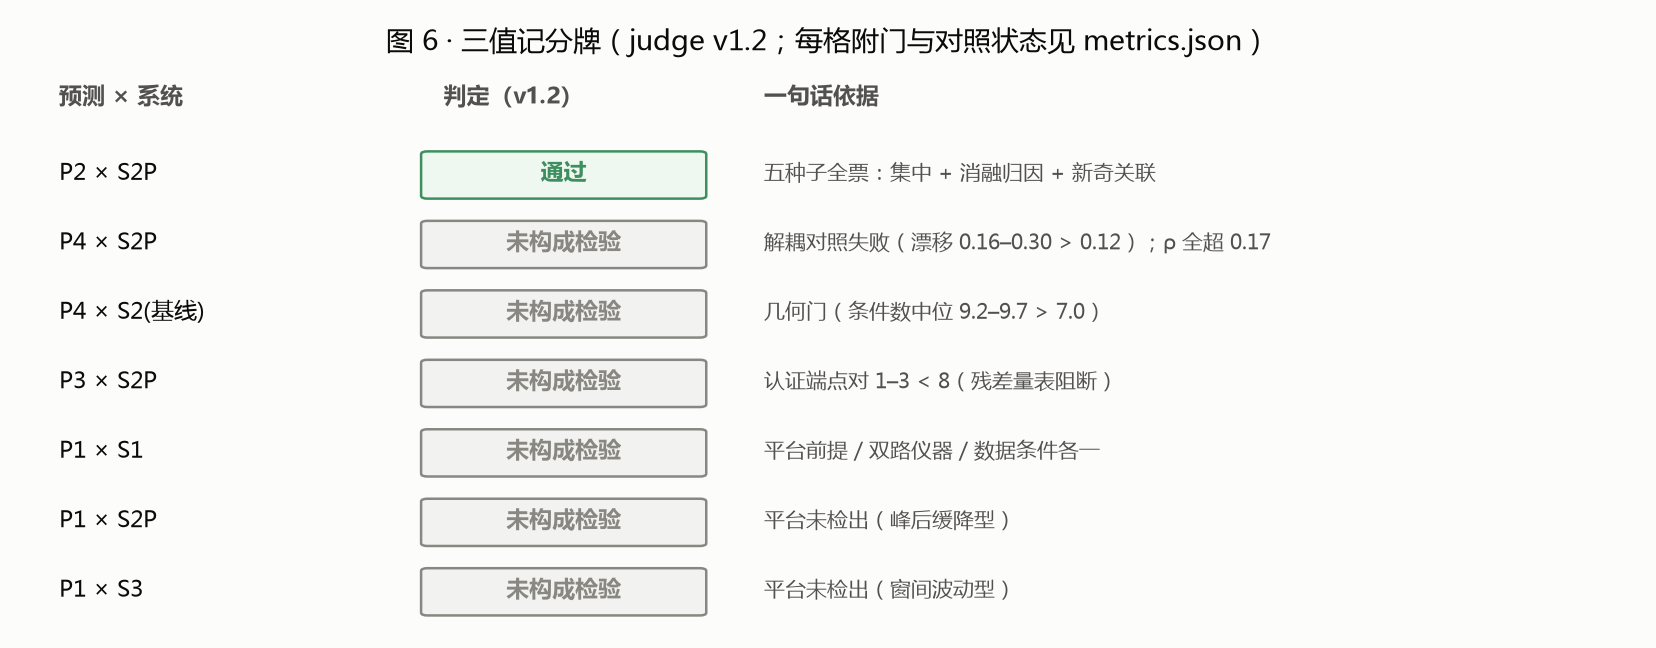
\includegraphics[width=0.86\linewidth]{../figures/fig6_scoreboard.png}
\caption{Three-valued scoreboard (judge v1.2). [Figure labels to be regenerated
in English for submission.]}
\label{fig:scoreboard}
\end{figure}

\subsection{The P2 pass: evidence chain (main result)}

System S2P, five evaluation seeds, $1000$ inference trajectories per seed, each
matched to $50$ metric-space smooth-random surrogates (matched in length and in
speed distribution under $\hat g$; the Euclidean surrogate was shown in
calibration to give a spurious full separation through kinetic mismatch, and is
discarded). All three layers pass (Figure~\ref{fig:p2}).
\begin{itemize}
\item \textbf{Concentration}: the fraction of trajectories whose $\hat
A_{\mathrm{OM}}$ median is below the lower quartile of the surrogate distribution
is $1.000$ on all five seeds (decision line $0.75$); the standardized-gap median
is $0.45$--$0.49$.
\item \textbf{Potential-term ablation} (validity core): setting $\nabla\hat V$ to
zero and rescoring the same paths gives a per-trajectory paired difference
(with-potential gap minus constant-potential gap) with median $+0.0021$ to
$+0.0036$ and Wilcoxon signed-rank $p$ between $1.0\times10^{-12}$ and
$6.9\times10^{-34}$---the with-potential version is systematically more
discriminating, so the concentration can be attributed to potential structure.
This criterion was flagged high-risk at pre-registration (on the base system S2
the gradient fraction was zero and the ablation had no power); on S2P it gains
power, and in step the empirical-drift gradient fraction changes from $0.000$ to
$0.04$--$0.11$.
\item \textbf{Novelty association and placebo}: the logistic regression of the
per-step action increment at novelty-injection steps (maze topology switch) on
the novelty indicator has a likelihood-ratio $p$ between $5.3\times10^{-7}$ and
$3.3\times10^{-4}$ with a positive coefficient; the placebo (random time shift of
the injection) is non-significant on all seeds ($p\ \,0.17$--$0.93$).
\end{itemize}
Following the pre-registered wording, the support here can only be stated as:
the observation is consistent with the hypothesis, and the increment beyond a
trivial explanation is---the concentration cannot be reproduced by kinetically
matched random paths (the surrogate already matches the speed distribution), nor
by a constant potential (the ablation paired difference is positive and
significant).

\begin{figure}[t]
\centering
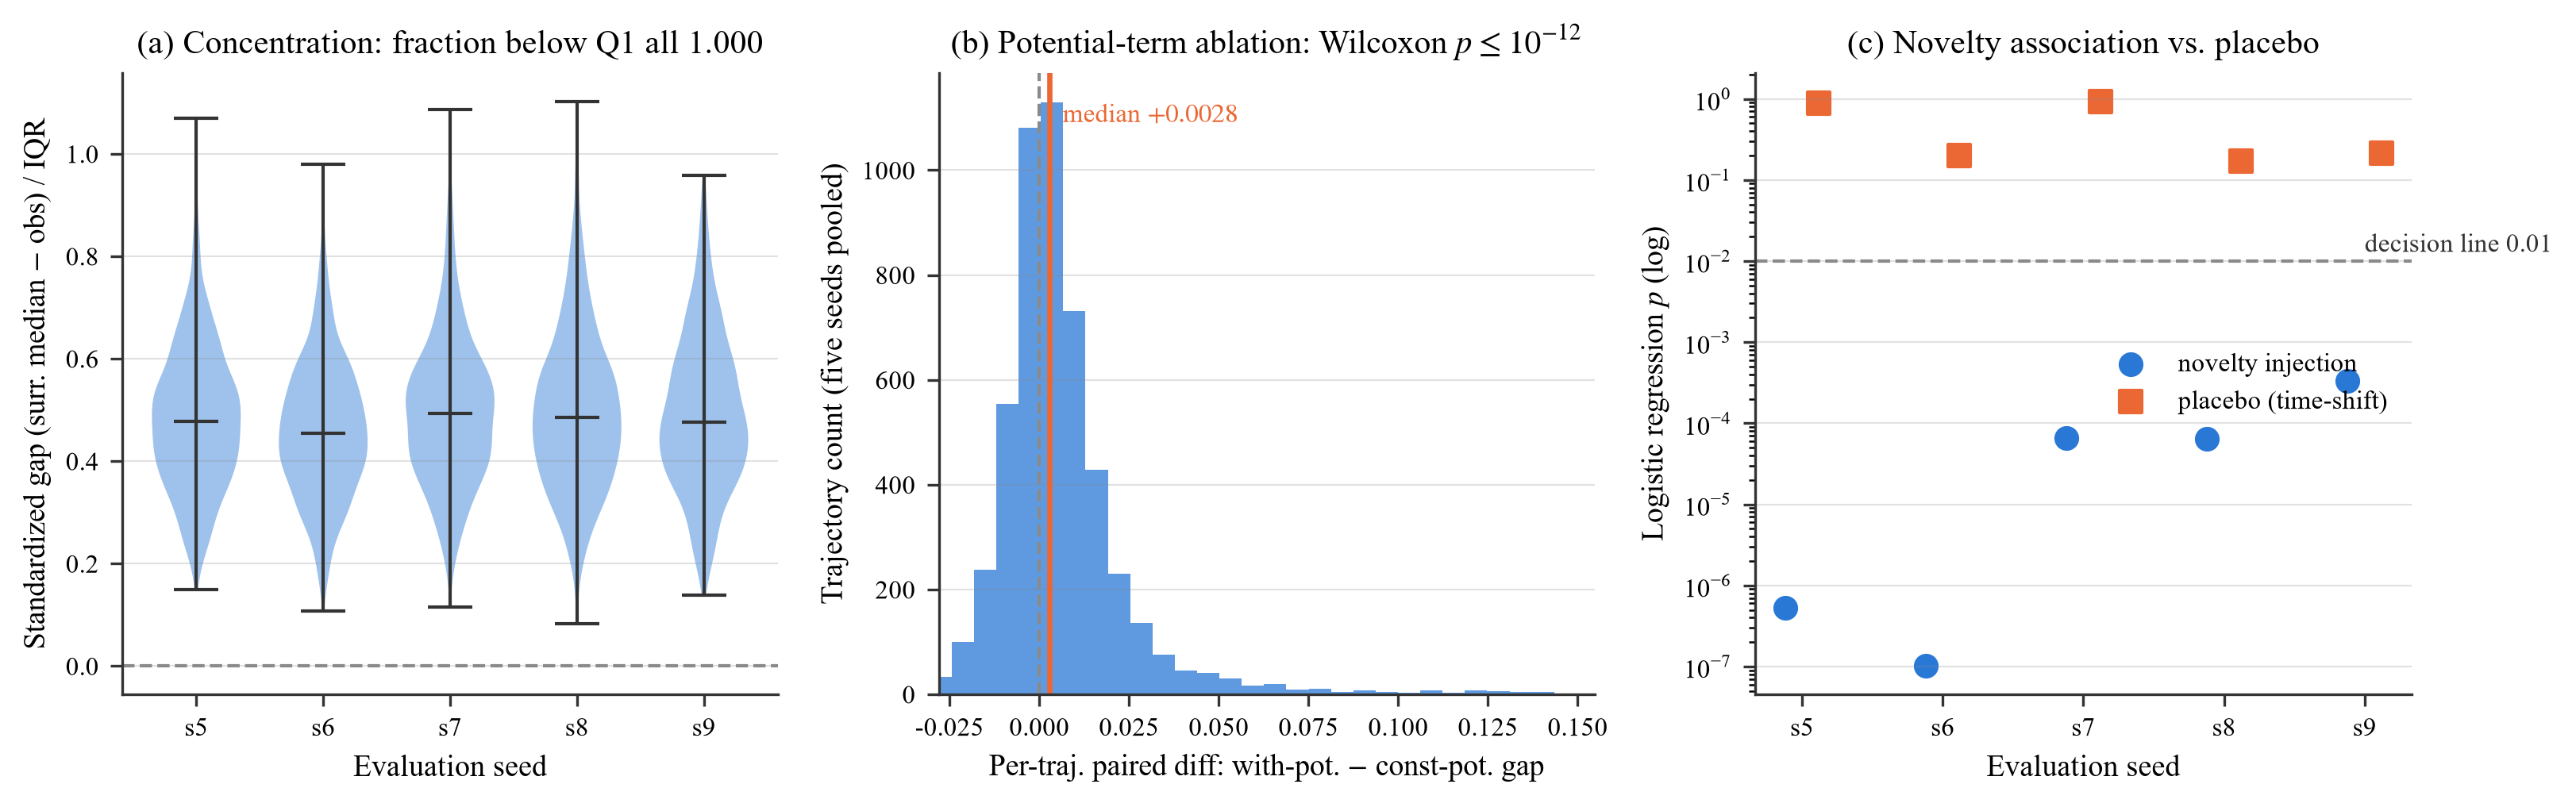
\includegraphics[width=\linewidth]{../figures/fig3_p2.png}
\caption{P2 $\times$ S2P (pass), three decision layers: concentration,
potential-term ablation, novelty association vs.\ placebo.}
\label{fig:p2}
\end{figure}

\subsection{P4: why the apparent affine law does not constitute support}

On S2P the instrument resolution is adequate: $R^2$ is $0.464$--$0.589$ (floor
$0.25$), the slope is consistent across seeds ($0.023$--$0.026$, i.e.\ $\hat T\
38.4$--$43.2$), the split-half temperature relative difference is
$0.028$--$0.109$ (tolerance $0.20$), and the multi-chain stationarity $\hat R \le
1.003$. Two layers nonetheless object (Figure~\ref{fig:p4}).
\begin{itemize}
\item \textbf{Decoupling control} (validity core): retraining the decoder on
occupancy-uniform data with the visitation distribution unchanged shifts the
slope by $0.159$--$0.298$, exceeding the tolerance $0.12$ on all five
seeds---a substantial part of the apparent affine law comes from ``the decoder
fits better where it is visited more,'' so by the pre-registered rule the
apparent affine law does not constitute support. A control on the control:
swapping the exploration policy (frozen decoder) barely moves the slope
($0.001$--$0.091$), and the intercept shift in the manipulation check matches the
predicted signature (ratio $0.99$--$1.01$), locating the failure in
decoder--occupancy coupling rather than in a pipeline bug.
\item \textbf{Curvature}: lack-of-fit statistically rejects ($p\le 10^{-26}$) and
the curvature effect size $\rho = |c|\cdot\mathrm{SD}(\hat V)/|b|$ is
$0.175$--$0.412$, exceeding the substantive-bending bound $0.17$ ($c$ the
quadratic coefficient, $\mathrm{SD}(\hat V)$ the abscissa standard deviation).
Even had the decoupling passed, the verdict would be fail rather than pass.
\end{itemize}
The base system S2 fails the geometry gate under both protocol versions
(20k-step condition-number median $9.18$--$9.70$).

\begin{figure}[t]
\centering
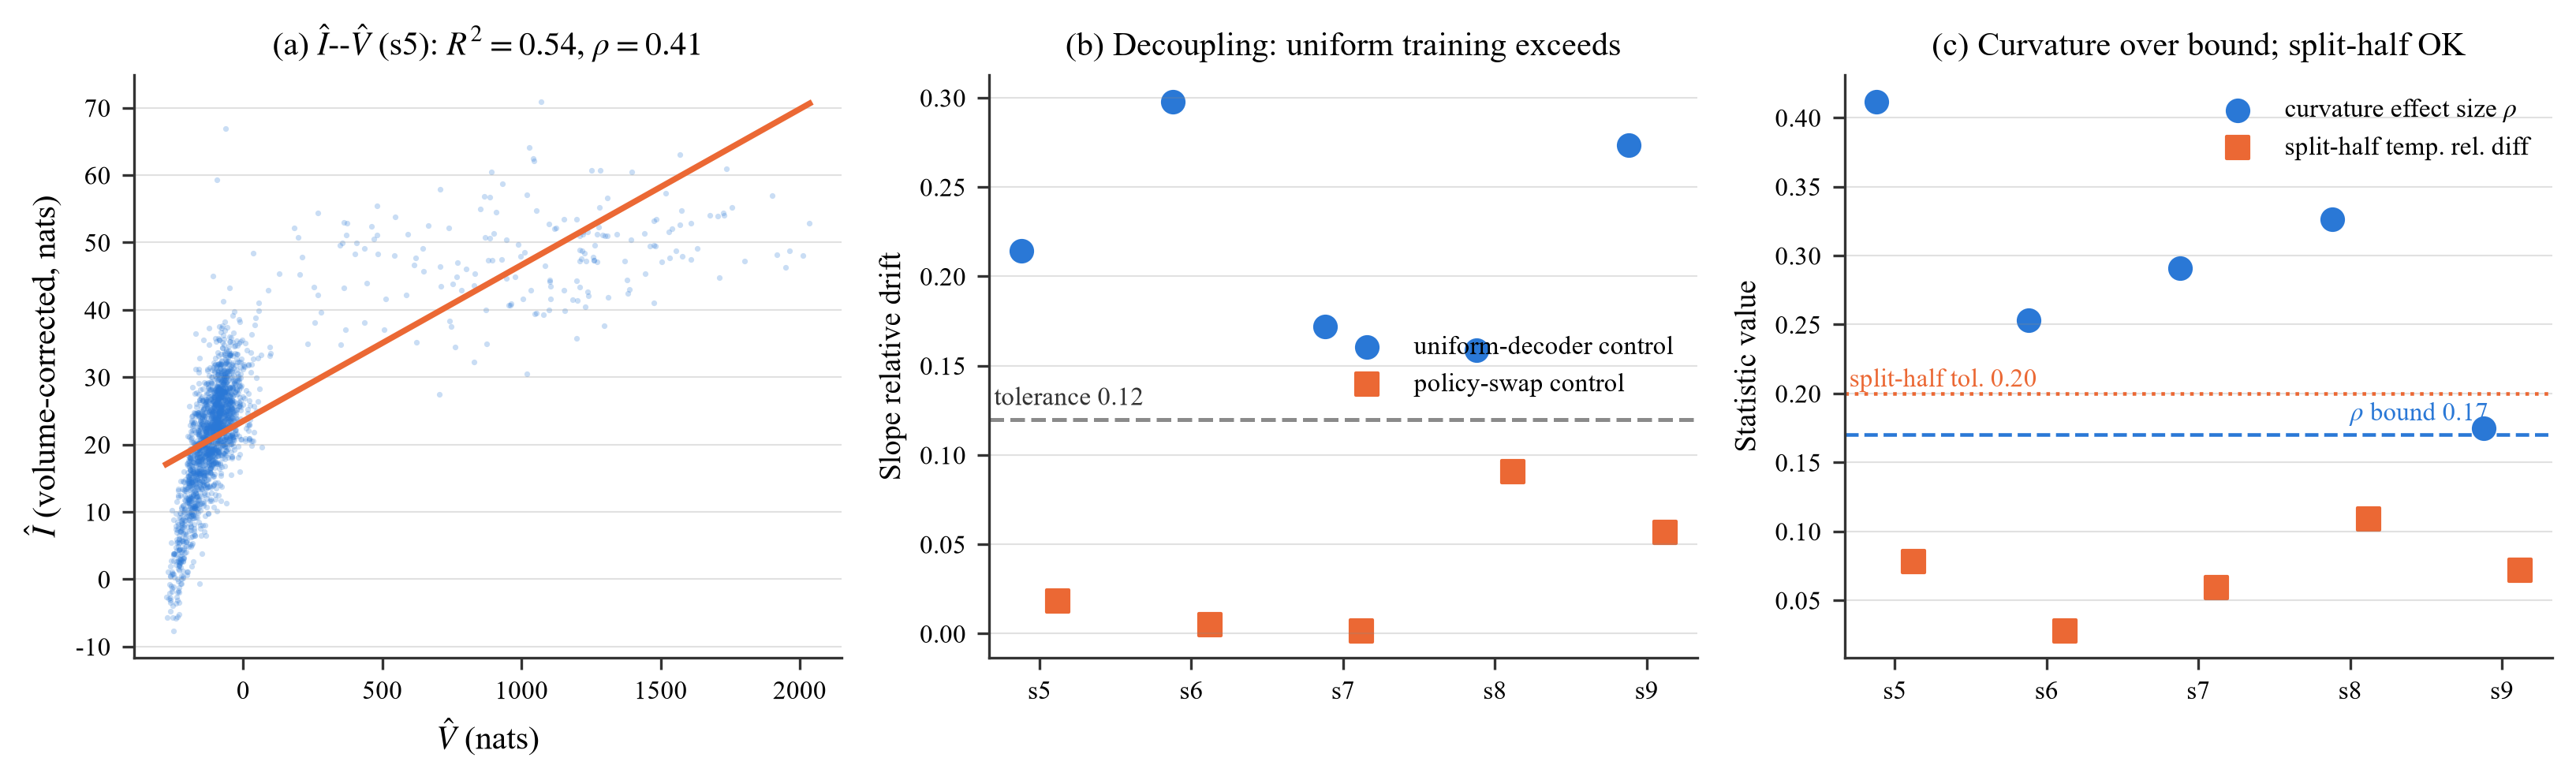
\includegraphics[width=\linewidth]{../figures/fig5_p4.png}
\caption{P4 $\times$ S2P (TNC): the instrument has resolution, yet the apparent
affine law does not constitute support. (a) $\hat I$--$\hat V$ scatter with fit;
(b) decoupling controls; (c) curvature $\rho$ over bound, split-half within
tolerance.}
\label{fig:p4}
\end{figure}

\subsection{P1: the plateau premise and post-peak entropy rise}

Across three architectures and thirteen gated training instances, no utility
plateau is detected by the frozen detector: the S1 escape instances are two
late-escape (still rising at the tail, the runtime window rule yielding a
window beyond the horizon) and one early-escape instance where the plateau is
detected but the entropy change is near zero relative to the noise band; S2P and
S3 give post-peak slow decline or window-scale wobble on all five seeds each. The
parent-paper layer premise does not hold and all are recorded as test not
constituted.

The supplementary peak-window layer (listed separately in the pre-registration
and not entering the title verdict) gives a directionally consistent reverse
signal (Figure~\ref{fig:p1}): within the window from the utility peak to twice
its position, the entropy change is $+1.3$ and $+1.9$ nats on S1, $-0.9$ to
$+9.3$ on S2P (four of five positive), and $+0.85$ to $+15.4$ on S3 (all
positive)---after utility tops out, entropy rises rather than falls more often.
This signal was observed already on the development family and pre-registered as
an ``expected-to-fail risky prediction''; the evaluation family reproduces it on
all three architectures. On S3 the dual-path entropy rank correlation is
$0.999$--$1.000$, the best instrument agreement, and the reverse signal is least
ambiguous.

\begin{figure}[t]
\centering
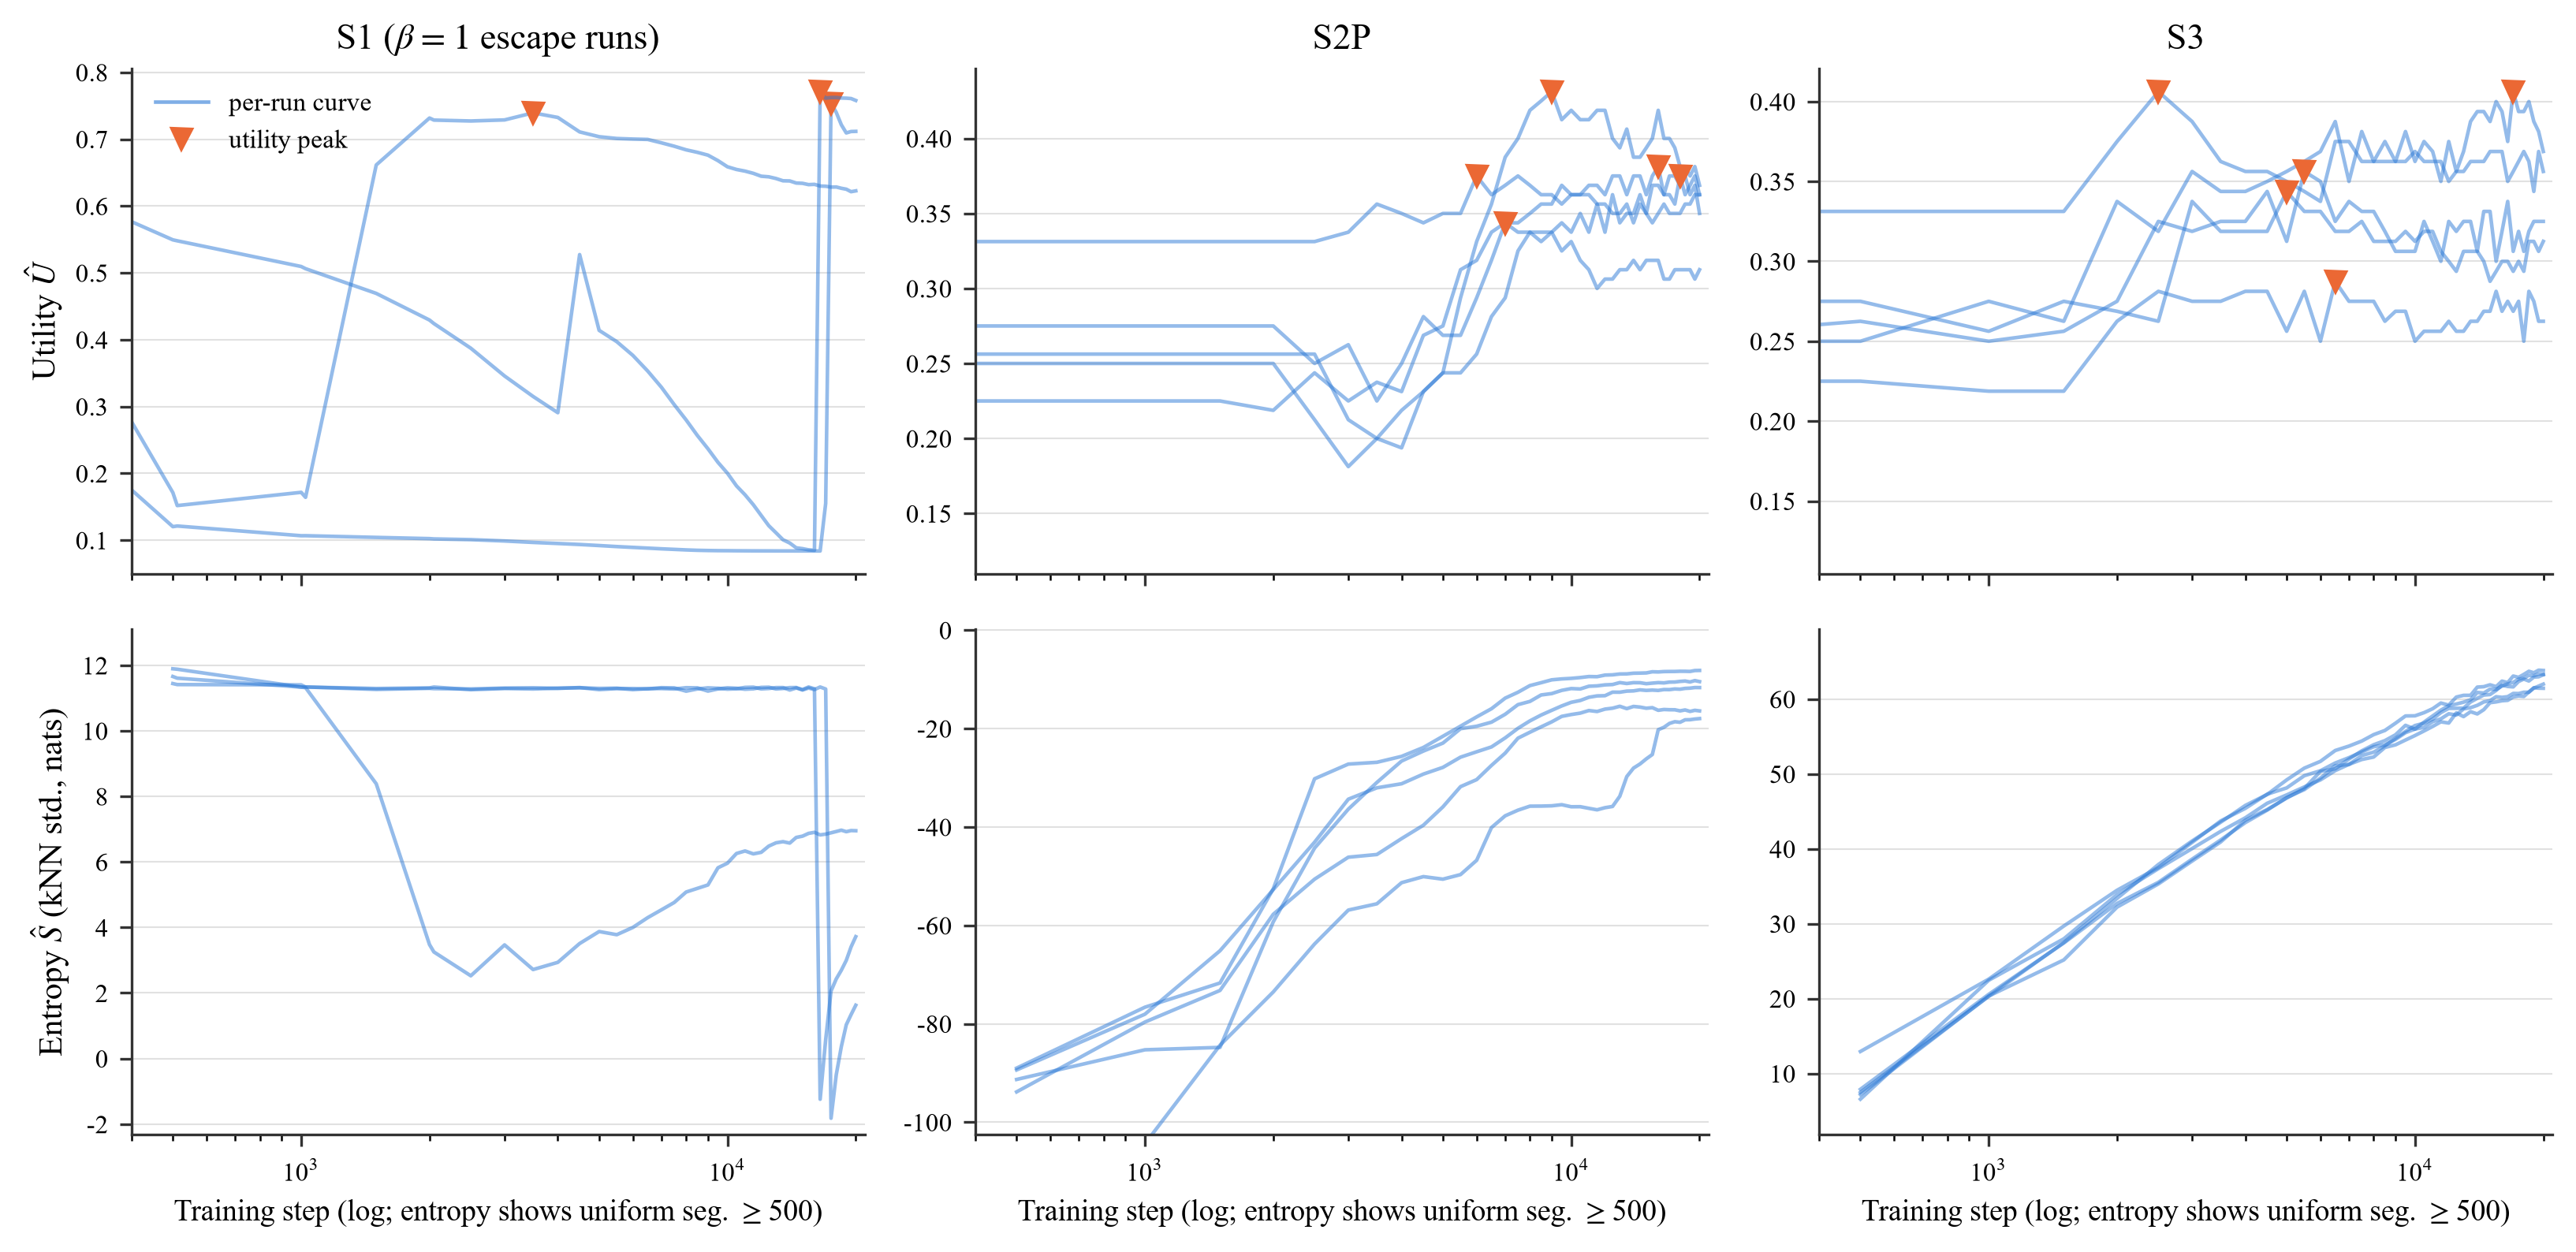
\includegraphics[width=\linewidth]{../figures/fig2_p1.png}
\caption{P1: utility and entropy along training on three architectures. Utility
tops out and entropy then rises (kNN standardized path; uniform segment only).
Plateau is detected on none.}
\label{fig:p1}
\end{figure}

\subsection{P3: why the test does not run}

The terrain gate is healthy (the bootstrap CI90 lower bound of the high/low
gradient tertile median ratio is $1.87$--$1.94$, so the terrain has detectable
structure), but the geodesic residual quality check rejects $70$--$77$ candidate
pairs per seed (of $76$--$80$ solved), leaving only $1$--$3$ certified (floor
$8$). The root cause is scale non-portability: the residual threshold $3\times
10^{-3}$ is calibrated on an analytically smooth synthetic metric, whereas on the
estimated MLP decoder metric the achievable residual is only about $0.26$ after
double precision, energy normalization, and an increased iteration budget
(Section~\ref{sec:scale}). P3 is recorded as test not constituted; the residual
scale non-portability is in Section~\ref{sec:scale}. See Figure~\ref{fig:p3}.

\begin{figure}[t]
\centering
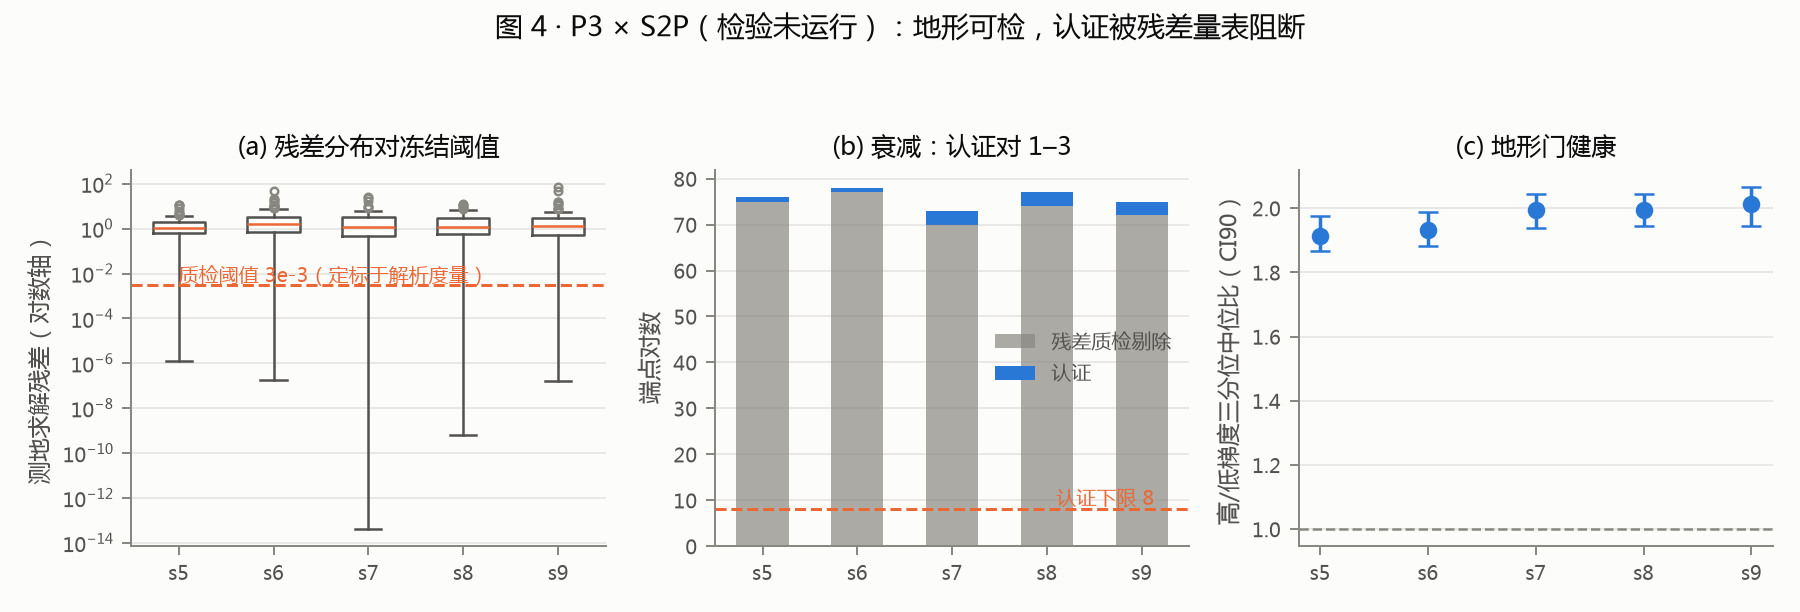
\includegraphics[width=\linewidth]{../figures/fig4_p3.png}
\caption{P3 $\times$ S2P (test not constituted): the terrain is detectable, but
certification is blocked by the residual scale. (a) residual distribution vs.\
frozen threshold; (b) attrition; (c) terrain-gate health.}
\label{fig:p3}
\end{figure}

\subsection{Four mechanisms behind ``test not constituted''}
\label{sec:tnc}

Three-valued accounting separates \emph{test not constituted} from \emph{fail}.
The epistemic difference is: a fail means the instrument works, completes the
measurement, and the result contradicts the prediction; a test not constituted
means the instrument cannot reach the question being asked on that system. The
six TNC cells here are not one situation. Sorted by where in the chain the
instrument falls short, they form four classes, and the classification itself
delineates the measurable boundary of the current estimators.

\emph{(i) Rejected at the gate (measurement never happens).} P4 $\times$ S2
(base): the condition-number median is $9.18$--$9.70$, far above the geometry
gate $7.0$, participation dimension $1.87$--$2.04$. The system leaves the
calibration-verified measurable region (Section~\ref{sec:calib}, feasibility
bound $7.0$) before any P4 statistic is computed; the affine fit never runs on a
meaningful geometry. This class is entirely neutral about the parent theory---it
only says this system at this training length is beyond the instrument's range.

\emph{(ii) Vetoed by a validity control (measurement happens but is shown
invalid).} P4 $\times$ S2P: resolution is adequate ($R^2\ 0.464$--$0.589$,
split-half $0.028$--$0.109$), but the decoupling control removes the apparent
affine law's standing---after retraining the decoder on occupancy-uniform data
the slope shifts by $0.159$--$0.298$ on all five seeds ($>0.12$), while swapping
the exploration policy barely moves it ($0.001$--$0.091$). Alongside, the
curvature effect size $0.175$--$0.412$ exceeds the bound $0.17$ on every seed.
This class is also essentially neutral about the parent theory: it says the
current estimators cannot decouple the self-information--potential relation from
the decoder's visitation statistics, not that the affine law is refuted.

\emph{(iii) Instrument reach short (the estimator cannot meet the quality
check).} P3 $\times$ S2P: the terrain gate is healthy (CI90 lower bound
$1.87$--$1.94$), but the geodesic residual check rejects $70$--$77$ pairs per
seed (of $76$--$80$ solved), leaving $1$--$3$ certified, below the floor $8$. The
root is scale non-portability: the threshold $3\times10^{-3}$ is calibrated on an
analytically smooth synthetic metric, and on the estimated MLP metric the
achievable residual is about $0.26$ (Section~\ref{sec:scale}). Terrain
measurable, pairwise geodesic not; the test does not run. This class is likewise
neutral about the parent theory, pointing at the geodesic solver's resolution on
estimated metrics rather than at whether low-gradient regions are near-geodesic.

\emph{(iv) Premise not met (no ground for the parent-paper layer).} P1 $\times$
S1/S2P/S3: the parent-paper layer requires post-plateau energy compression, and
the plateau premise holds on none of the thirteen gated training instances. S2P
and S3 detect no plateau on all five seeds each (tail noise $\hat\sigma_{\rm rel}\
0.003$--$0.008$, runtime window $W=3$, no three consecutive flat windows). The
three gated S1 escape instances hit three different instrument limits: one with
no plateau detected (parent-paper premise), one failing the dual-path entropy
shape criterion (rank correlation $<0.9$), one exceeding the CAL-P1 data
condition on $\sigma_{\hat U}$. Unlike the first three classes, this one carries
information about the parent theory: the supplementary peak-window layer gives a
directionally consistent reverse signal on the measurable instances (entropy
change $+1.3$ and $+1.9$ on S1, $-0.9$ to $+9.3$ on S2P, $+0.85$ to $+15.4$ on
S3)---after utility tops out, entropy rises rather than falls. The signal was
pre-registered on the development family as an expected-to-fail risky prediction
and reproduces on the evaluation family across three architectures; on S3 the
dual-path rank correlation $0.999$--$1.000$ makes it least ambiguous.

In sum, of the six TNC cells five (the two P4 cells, the P3 cell, and the
gate/instrument/data-condition subcells of P1) delineate instrument boundaries
and are neutral about the parent theory's truth; only ``P1 parent-paper premise
not met'' carries negative information, and its supplementary-layer post-peak
entropy rise is a stable phenomenon that calls for a theoretical response. We
state this classification explicitly so that ``test not constituted'' is not
misread as ``tested but inconclusive'' or as ``a disguised failure''---each cell
delineates a specific instrument or premise boundary.

\section{Instrument findings}
\label{sec:instr}

\subsection{Mutual exclusion of training length and metric measurability}
\label{sec:geomexcl}

The S2 base condition-number median grows monotonically with training: about
$2.4$--$2.9$ at $500$ steps, crossing $6.0$ at $6000$--$8000$, reaching
$9.0$--$9.6$ at 20k with no sign of saturation; yet the utility plateau appears
around 15500 steps. Learning to predict the target well requires pushing the
decoder into the sigmoid saturation region, and saturation makes some hidden
dimensions invisible to the observation geometry---the utility-plateau region and
the measurable region ($\le 7.0$) do not intersect on this system. An
equal-variance control shows the condition number is unrelated to the
per-channel variance design and comes entirely from decoder-Jacobian degeneracy.

\subsection{Order-of-magnitude repair by a multi-step decoder head}
\label{sec:multistep}

Diagnosis attributes the low end of the condition number to hidden memory
dimensions the decoder does not use (the instantaneous observation does not
depend on them). Letting the decoder head output the concatenation of the next
four observations makes the memory dimensions visible to the predictive
observation geometry: the S2P condition-number median drops to $2.95$--$3.09$
(six orders of magnitude), with no hardening throughout, and utility is not hurt
(evaluation-family peak $0.368$ vs.\ base $0.329$); the same repair pulls S3 back
from a near-rank-one degeneration (condition number $10^{28}$, participation
dimension $1.0$) to $4.2$--$4.4$. The drift gradient fraction changes from
$0.000$ to $0.04$--$0.11$, and the P2 potential-term ablation goes from no power
to strong power---the P2 pass is in effect unlocked by this instrument repair.

\subsection{Feasibility is not a single-variable function of the condition
number}

A transplant experiment in the feasibility-boundary refinement: at the same
condition number (the $5.74$ bin), replacing only the synthetic system's
potential-well stiffness spectrum from a log-uniform ladder with a random draw
containing near-duplicate values degrades the temperature recovery error from
about $8\%$ to about $39\%$, the failure running through the potential
estimation. Two systems with the same metric-spectrum statistics can have
sharply different feasibility---the condition-number gate is a necessity screen,
and a sufficiency certificate can only come from a per-system geometry-matched
calibration recovery.

\subsection{Residual scale and criterion portability}
\label{sec:scale}

Two criteria lose scale when transplanted from the synthetic calibration system
to the real estimated system: the geodesic residual (Section on P3) and the P1
dual-path sign criterion (sign disagreement on a near-zero change carries no
information; v1.2 adds an amplitude floor, in the direction of making the test
stricter). Aligning the scale between the calibration system where a threshold is
set and the application system where it is used should be an explicit check in
the calibration phase.

\section{Evidence grade and limitations}

\begin{itemize}
\item \textbf{Two protocol versions}: v1.1 is the original pre-registration; v1.2
was amended after the evaluation-family aggregate results were public, so the
verdicts under it (including the single pass P2 $\times$ S2P) are at the
``pre-registration after revision'' grade. The amendment criteria do not look at
the direction of prediction success (the geometry-gate recalibration depends only
on synthetic ground-truth recovery), and the S2P design uses only
development-family data, but the evaluation seeds $\{5$--$9\}$ were used for the
base-system S2 experiments, so information exposure at the aggregate-statistic
level exists while per-task-level leakage does not. This is an inherent cost of
the revision route, recorded honestly.
\item \textbf{Boundary of the P2 pass cell}: the ablation paired difference is
numerically small ($0.002$--$0.004$ standardized-gap units), its significance
coming from the consistent direction over $1000$ pairs; the novelty association
is a consistency check rather than a mechanism proof; under the rank convention
with $T=1$, P2 does not depend on $\hat T$ identification, but for the same
reason it cannot conversely support P4.
\item \textbf{Scope statement} (parent protocol Section~13): the measured energy
is a dimensionless form of the reconstruction cost defined by the decoder, and
whether it deserves to be called ``semantic'' is exactly what is under test; we
do not presume it. Non-stationary environments and cross-modal prediction (P5)
are outside the scope of this paper.
\item The systems are small (latent dimension $\le 16$, single-machine CPU
scale); the extrapolation of the conclusions is untested.
\end{itemize}

\section{Conclusion}

The accounting of the four predictions within the measurable range: one passes
(P2, low-action concentration, with potential-structure attribution), one is
objected to on two layers under an instrument with resolution (P4), one has its
premise not hold on three architectures with a stably reproduced reverse signal
(P1), and one does not run because of residual-scale non-portability (P3). The
three tests-not-constituted differ in epistemic weight (Section~\ref{sec:tnc}):
the P4 and P3 ones are instrument boundaries, neutral about the parent theory's
truth; only ``P1 parent-paper premise not met'' carries negative information. The
implications for the parent theory are stated accordingly: the inference-scale
``trajectories concentrate on low-action paths'' obtains support beyond a trivial
explanation; the learning-scale ``compression after fit'' does not appear on any
system here, and the post-peak entropy rise is a stable phenomenon calling for a
theoretical response; the affine law and temperature identification cannot be
decoupled from the decoder-occupancy effect under current estimator technology,
so we make no positive or negative judgment on the affine law and its test
validity depends on instrument improvements that do not yet exist.

\section*{Reproducibility statement}

The public repository (anchor commits \texttt{f7f7910} for v1.1 and
\texttt{27df5af} for v1.2) contains all code, configurations, judging artifacts,
and both frozen manifests. Seed families (calibration $\{99,100\}$, development
$0$--$4$, evaluation $5$--$9$) are mechanically enforced by a guard that blocks
the evaluation family before the freeze flag is set. The verdict file
\texttt{metrics.json} is written only by the frozen judging code. The estimator
toolbox is released with the repository as a public citation anchor. (The
repository URL is withheld here for the anonymous submission.)

\bibliographystyle{tmlr}
\bibliography{references}

\end{document}
